\subsection{Carte du jeu}

\vspace{0.5cm}
\subsubsection{Cahier des charges}
\vspace{0.5cm}

    \paragraph{Taille et topologie de la carte}
        
        La carte du jeu doit être parfaite. En effet, toutes les mécaniques 
        (saut, échelles, course)
        deviennent inutiles si elles sont implémentées sur une carte inadéquate (avoir la 
        possibilité de grimper sur une carte plate est aussi inutile que frustrant).
        A l'inverse, une carte adaptée aux possibilités de déplacement du joueur donne à ce dernier
        l'impression de quelque chose de fini.
        Une carte spacieuse et assez verticale (accidentée et/ou avec des maisons escaladables)
        se présente donc comme la meilleure option, car elle est ainsi le moins restrictive possible.


    \paragraph{Univers et design}

        Le jeu se déroule dans un univers pirate, aux Caraïbes.
        Les bâtiments doivent donc être d'inspiration hispanique,
        mais paraître peu entretenus, signe d'une longue occupation 
        pirate. La carte est une île, ce qui permet de justifier
        la limite de carte facilement (océan). En revanche, certaines 
        incohérences (skin de squelette, peut être des armes futuristes)
        permettent d'inscrire le jeu dans un registre informel, et de 
        rappeler que ce n'est qu'un jeu.


        \begin{figure}[!hbt]
            \centering
            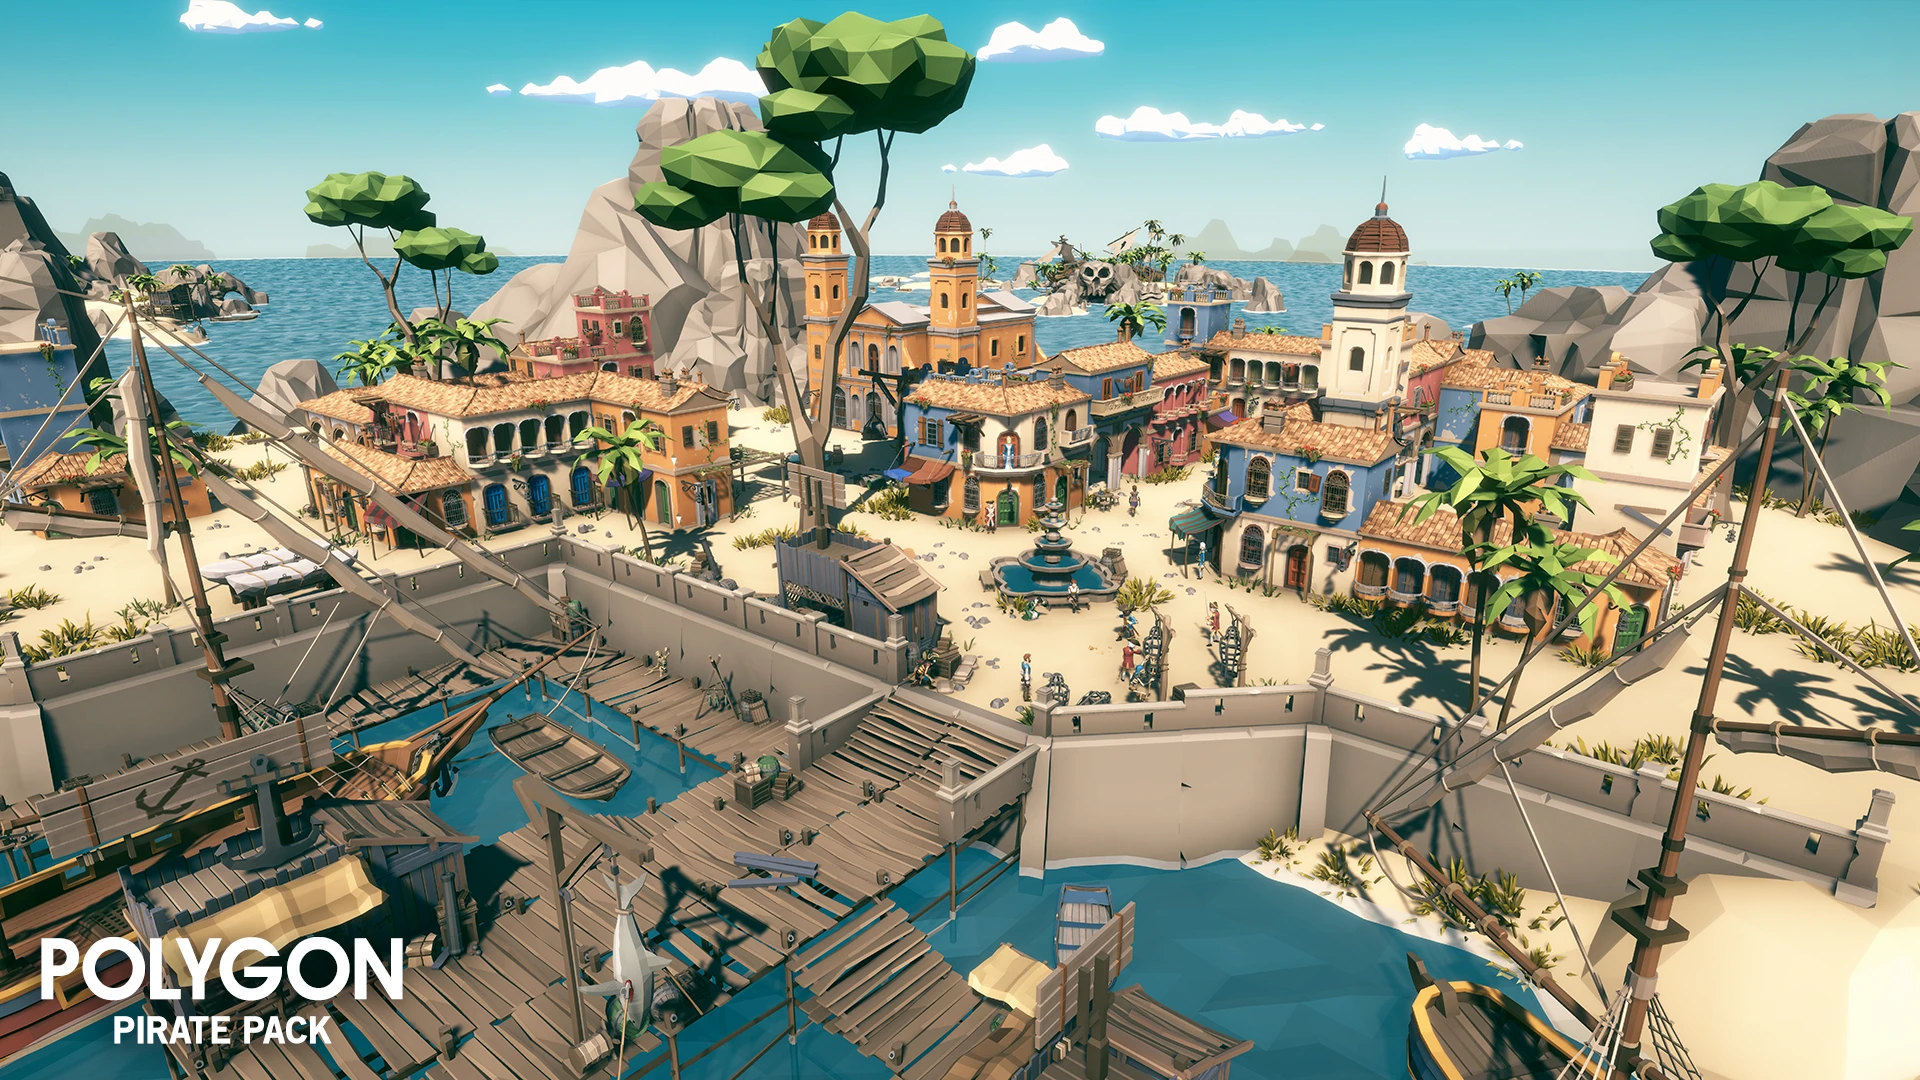
\includegraphics[scale=0.18]{polygon_pirate.png}
            \caption{Image de présentation de l'asset Polygon Pirate}
        \end{figure}


    \paragraph{Assets}

        Tous ces éléments nous ont fait opter pour l'achat d'un asset graphique chez 
        Synty Studios (POLYGON - Pirate Pack).
        Ce dernier possède de nombreux avantages, comme sa grande diversité de prefabs et 
        textures, ou encore son aspect "Low Poly", 
        c'est-à-dire en polygones, qui donne un aspect moderne au jeu tout en diminuant la 
        complexité des mesh (réduisant ainsi la 
        puissance de calcul nécessaire au jeu).
        

\vspace{0.5cm}
\subsubsection{Première soutenance}
\vspace{0.5cm}

    La carte étant un élément crucial du jeu, au même titre que les mécaniques, 
    il nous a semblé important de faire des schémas et que le groupe soit d'accord sur la direction artistique,
    afin que Paul, la personne en charge de la map, puisse être sûr de la vision de la carte du jeu avant de commencer.
    commencer. Ainsi, la carte finalement retenue devait avoir suffisamment de 
    relief pour rendre les échelles intéressantes, et suffisamment spacieuse pour 
    pouvoir la remplir avec au moins 150 personnages non-joueurs (afin de pimenter le jeu).
    Dans un premier temps, une forme ronde avait été retenue pour la carte, mais 
    a ensuite évolué pour une forme en L, cette dernière rendant l’environnement 
    plus naturel et augmentant les chances des personnages de se croiser.

    \begin{figure}[hbt!]
        \centering
        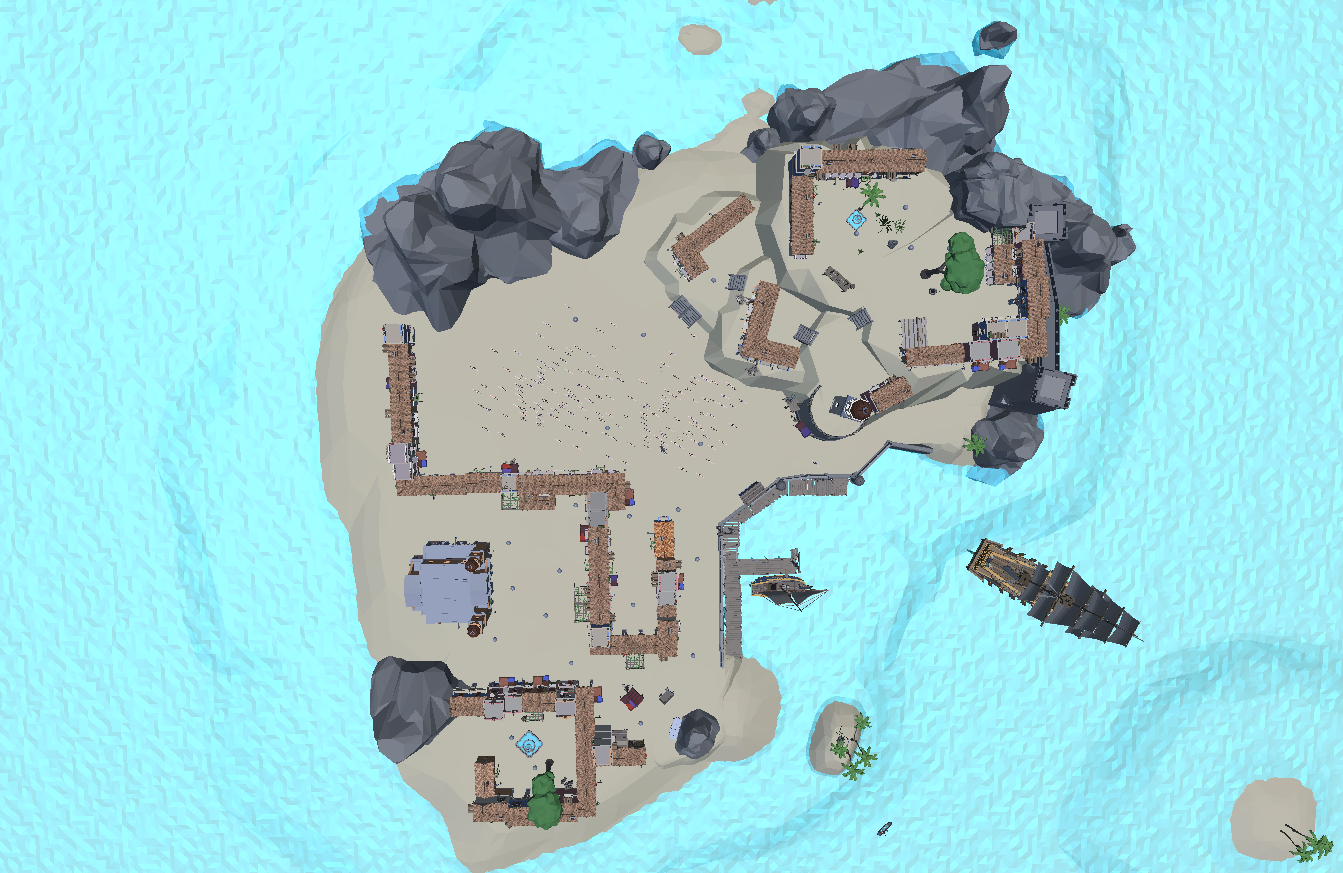
\includegraphics[scale=0.42]{fly_view.png}
        \caption{Vue aérienne de la carte}
    \end{figure}
    \FloatBarrier

    Ensuite, afin d’ajouter du relief à la carte, une colline a été créée. 
    Cette dernière s’étend sur environ un quart de la carte, et possède quatre 
    niveaux afin d’en permettre l’accès par de petits escaliers successifs. 
    Une colline étant un terrain irrégulier, il a été décidé que les bâtiments 
    placés sur cette dernière ne seraient pas parallèles, mais répartis afin de 
    créer un imbroglio de maisons rappelant le style méditerranéen dont les îles 
    comme celle-ci sont inspirées.
    

    \begin{figure}[hbt!]
        \centering
        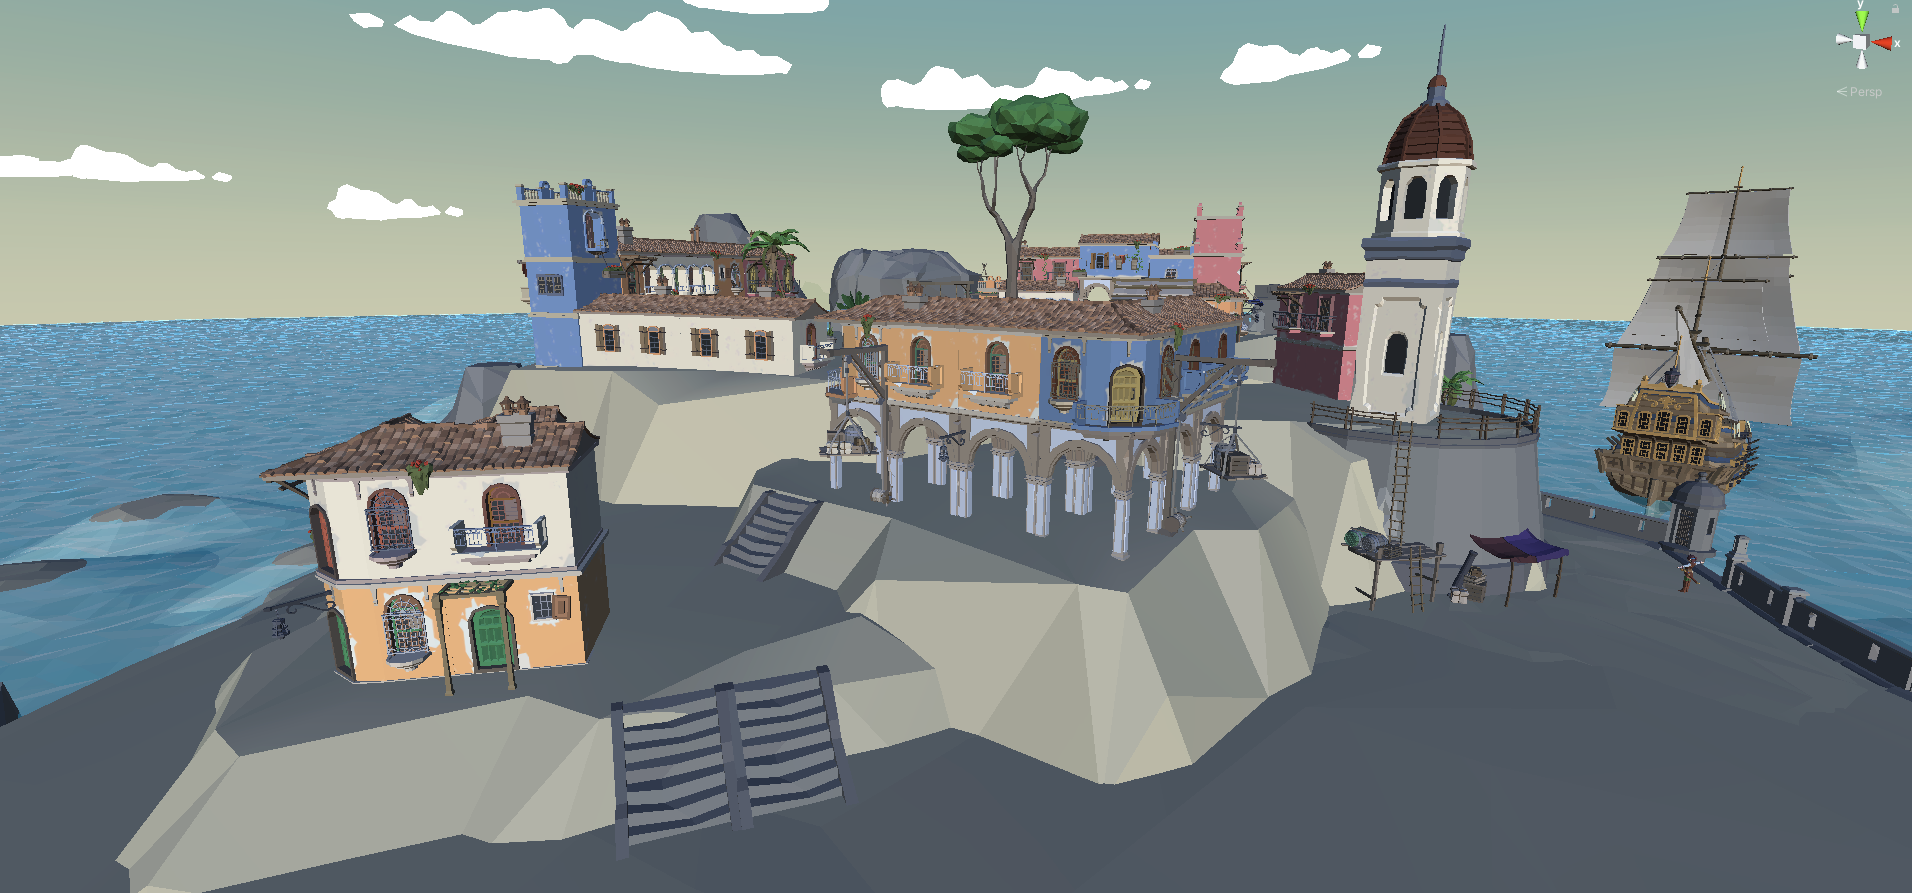
\includegraphics[scale=0.29]{hill.png}
        \caption{Colline de la carte, organisée par étages}
    \end{figure}
    \FloatBarrier

    Enfin, l’architecture de la ville elle-même devait aussi avoir une influence 
    ibérique, les maisons ont été dessinées basses et organisées autour de places et 
    marchés animés. Les tonnelles et les nombreuses lanternes rendent l’environnement 
    plus chaleureux, et les arcades, dotées de portes qui se ferment lorsqu’un joueur 
    les passe en courant, ajoutent une mécanique de fuite au jeu\footnote{Cf. Gameplay/Environnement}. L’organisation du 
    village se fait autour de la place de l’église, qui fait office de place du marché.

\vspace{0.5cm}
\subsubsection{Deuxième soutenance}
\vspace{0.5cm}

    La carte est désormais finie, et de nouveaux éléments ont été ajoutés, comme un shader animé (créé avec l'outil Shader Graph) pour l'eau,
    faite par Dov, ou encore de nouvelles lumières dynamiques. Elle est aussi dotée de nombreuses échelles, qui permettent de fuir ses poursuivants 
    de façon discrète, ainsi que de venelles reliant les avenues.
    En outre, les nombreux NPC ainsi que les marchandises exposées au milieu des rues font aussi de bonnes diversions.
    Enfin, l'ajout d'escaliers offrant un second accès à la colline permettent non seulement de désengorger la butte, envahie par les NPC, mais aussi 
    de redynamiser la digue qui était jusque là exempte de tout intérêt : pas de bâtiments, pas de cachettes...
    
    Mais la principale nouveauté est le mode nuit : en effet, il est désormais possible de passer du jour à la nuit grâce à de simples boutons-radios. 
    Le mode nuit applique des effets de post-processing à toutes les textures de la carte, et assombrissant les couleurs et en appliquant certains effets 
    visuels se traduisant en jeu par un environnement plus sombre (deonc nocturne). 
    Ce mode nuit permet de faire ressortir la beauté de la ville endormie, tout en ajoutant un côté angoissant aux parties,
    qui deviennent \textit{de facto} beaucoup plus animées.
    Il reste à peaufiner les détails, comme l'ajout de hautes herbes dans les rues, le placement de torches utilisant 
    la lumière dynamique (mode jour / nuit) ou encore le réajustement de petites erreurs de placements.

\vspace{0.5cm}
\subsubsection{Dernière soutenance}
\vspace{0.5cm}

    \paragraph{Nouvelle carte}

    Une deuxième carte a été commencée, afin d'ajouter de l'intérêt au jeu. Cette dernière utilise le fort de la carte 
    de démonstration de l'Asset (faite par Synty), que nous avons modifié, en ajoutant de nombreuses rampes d'accès ainsi qu'une tyrolienne \footnote{Cf. Mécaniques de jeu}, 
    le nouveau mode de déplacement du jeu. Le quartier de pêcheurs sur la plage permet de créer une zone "urbaine", pour se 
    cacher dans la foule, alors que le fort permet de prendre de la hauteur pour repérer sa cible. Une grande difficulté rencontrée sur 
    cette carte est sa verticalité, qui requiert un nombre important d'escalier et de rampes d'accès, pour permettre la 
    circulation des joueurs mais surtout des NPC dont les reègles de circulation sont très strictes (restrictions sur l'inclinaison 
    du sol, sur la hauteur de saut et sur les objets de sol). L'accès au fort a dû être fortement restreint afin de ne garder 
    que les parties les plus accessibles (parvis et cour intérieur).

    \begin{figure}[hbt!]
        \centering
        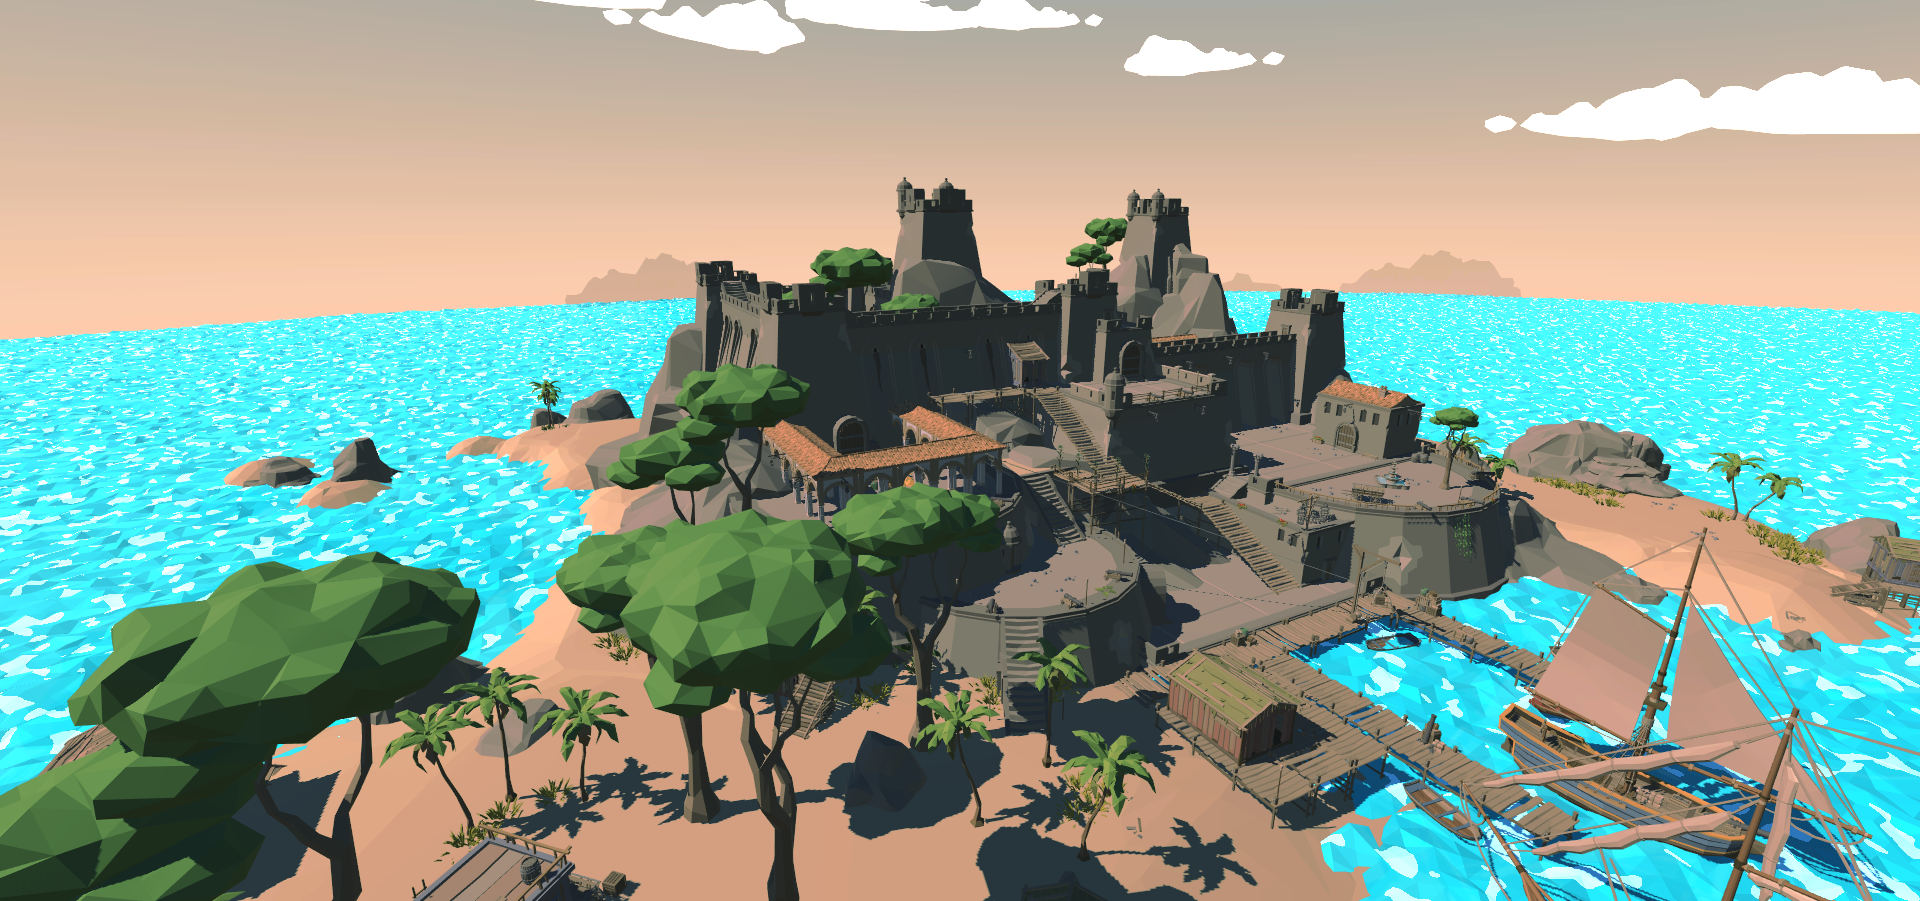
\includegraphics[scale=0.22]{second_map.png}
        \caption{Vue aérienne du fort de la seconde carte}
    \end{figure}
    \FloatBarrier


    \paragraph{Finition de la première carte}

    Une nouvelle tyrolienne ayant été créée, il nous a semblé impératif de l'ajouter à la carte. Il est donc maintenant possible 
    de grimper en haut de la grande tour, pour ensuite se laisser glisser sur une centaine de mètres. Des props ont aussi 
    été ajoutées, afin de rajouter du détail et donc du réalisme au jeu. Ces props consistent en des objets naturels (feuilles, pierres, 
    hautes herbes...) et en des petits objets, posés sur les tables du marché ou devant des maisons (tonneaux, pièces, boussoles...)
    Des murs invisibles, dont le franchissement est impossible autant aux joueurs qu'aux NPC, délimitent maintenant la limite 
    jouable de la carte, pour éviter toute forme d'antijeu de la part des joueurs et tout déplacement hasardeux des NPC.
    

    \paragraph{Ambiance sonore}

    Une grande nouveauté du jeu est l'ajout de sons d'ambiance, qui représentent une grande avancée. En effet, bien que cela soit 
    simple à implémenter grâce au composant \textit{source audio} d'Unity, les sons sont très importants pour casser 
    la monotonie du jeu. En effet, un joueur qui n'a pour sons que ses clics de souris a tendance à se lasser très vite, alors 
    que l'ajout de sons, même désactivables, dynamise le jeu.

    Des sons de vagues et de perroquets ont été téléchargés sur une bibliothèque de sons libres de droits, et ont été associés 
    à des objets de la carte. Dans le cas des bruits d'océan, ils ont dû être ajoutés à des objets invisibles situés près des 
    plages, afin d'éviter que toutes les tuiles d'océan jouent le son, ce qui serait aussi coûteux que désagréable. 
